\documentclass{beamer}

\usepackage[francais]{babel}
\usepackage[utf8]{inputenc}
\usepackage[T1]{fontenc}
\usepackage{graphicx}
\usepackage{graphics}
\usepackage{color}
\usepackage{textcomp}
\usepackage{pifont}
\usepackage[normalem]{ulem}
\usepackage{times}
\usepackage{hyperref}
\usepackage{verbatim}
\usepackage{amsmath}
\usepackage{amsthm}
\usepackage{amsfonts}
\usepackage[mathscr]{euscript}
\usepackage{pgfpages}
\usepackage{listings}
\usepackage{subfigure}
\usepackage{algorithm}
\usepackage[noend]{algorithmic}
\usepackage{pdftricks}
\usepackage{mathrsfs}
\usepackage{array}
\usepackage{fancybox}
% \usepackage{columns}
\usepackage{multirow}
\usepackage{url}
\usepackage{tikz}
\usepackage{colortbl}
%\usepackage{cite} %DO NOT FUCKING USE CITE ON BEAMER !!! LOST 30 GODDAM' MINUTES ON THIS SHIT !!!
\usepackage{mathabx}
\usepackage{amssymb}
\usepackage{eurosym}
\usepackage{wasysym} % ch0

\let\texteuro\euro

\hypersetup{colorlinks,%
            citecolor=black,%
            filecolor=black,%
            linkcolor=black,%
            urlcolor=blue}

%\addtolength{\parskip}{10pt}

\usetikzlibrary{calc}

\mode<presentation>
\setbeamertemplate{footline}[frame number]
\setbeamercovered{transparent}
\usetheme[navigation]{ESI}

%lst
\definecolor{comment-green}{RGB}{0,166,80}
\lstset{language=C++,
  keywordstyle=\lst@ifdisplaystyle\bf\fi\color{blue!60},
  commentstyle=\color{comment-green},
  stringstyle=\color{red},
  basicstyle=\lst@ifdisplaystyle\tiny\else\tt\fi,
  morekeywords={
    constexpr,concept,decltype,nullptr,nullptr_t,noexcept,final,override},
  frame=single,
  xleftmargin=0.5cm,
  numbers=left,
  tabsize=2}

%title
\subtitle{Langage \texttt{C} / \cpp}
\author{R. Absil}
\date{\today}

%styles
\theoremstyle{definition}
\newtheorem{thm}{Théorème}
\newtheorem{conj}[thm]{Conjecture}
\newtheorem{deff}[thm]{Définition}
\newtheorem{prop}[thm]{Propriété}
\newtheorem{lem}[thm]{Lemme}
\newtheorem*{lem*}{Lemme}
\newtheorem{cor}[thm]{Corollaire}
%\newtheorem{example}{Exemple}
\newtheorem{remark}{Remarque}
\newtheorem{exo}{Exercice}

%typeset
\newcommand{\ie}{{\emph{i.e., }}}
\newcommand{\eg}{{\emph{e.g., }}}
\newcommand{\etal}{{\emph{et al.}}}
\newcommand{\rrceil}{\unichar{"2308}}
\newcommand{\sloand}[2]{\footnote{N. J. A. Sloane - OEIS Foundation - \texttt{www.oeis.org}, Sequence #1 - #2.}}

%math
\newcommand{\IN}{{\mathbb N}}
\newcommand{\IQ}{{\mathbb Q}}
\newcommand{\IR}{{\mathbb R}}
\newcommand{\IZ}{{\mathbb Z}}
\newcommand{\IP}{{\mathbb P}}
\newcommand{\IC}{{\mathbb C}}
\newcommand{\bigo}{{\mathcal{O}}}
\renewcommand{\mod}{\bmod}
\newcommand{\ssi}{\Leftrightarrow}
\newcommand{\then}{\Rightarrow}
\newcommand{\fle}[1]{\stackrel{#1}{\longrightarrow}}
\newcommand{\suchthat}{~\big|~}
\newcommand{\floor}[1]{\left\lfloor #1 \right\rfloor}
\newcommand{\ceil}[1]{\left\lceil #1 \right\rceil}
\DeclareMathOperator*{\argmin}{argmin}
\DeclareMathOperator*{\argmax}{argmax}

%tikz
\tikzstyle{_vertex}=[fill=white, circle,minimum size=12pt,inner sep=1pt]
\tikzstyle{_blackv}=[fill=black, circle,minimum size=8pt,inner sep=1pt]
\tikzstyle{_dot}=[fill=black, circle, minimum size = 1mm, inner sep=0pt]
\tikzstyle{_bigvertex}=[fill=white, circle,minimum size=21pt,inner sep=1pt]
\tikzstyle{_arc}=[->, >=stealth]
\tikzstyle{_boldarc}=[->, >=stealth, line width=2pt]

\newcommand{\cpp}{\texttt{C++}}
\newcommand{\java}{\texttt{Java}}


\title{Ch. 2 - Pointeurs}

\begin{document}
\begin{frame}
  \titlepage
\end{frame}

\begin{frame}
  \frametitle{Table des matières}
  \footnotesize \tableofcontents[pausesections,pausesubsections]
\end{frame}


\section{Introduction}

\begin{frame}
\frametitle{Overview}
\begin{itemize}[<+->]
\item Les pointeurs sont utilisés comme des étiquettes pour désigner d'autres objets
\item On les utilise 
	\begin{itemize}
	\item si l'on veut propager en écriture des effets de bords (modifier un paramètre de fonction)
	\item si on ne veut pas que des copies implicites de données soient effectuées
	\end{itemize}
\item Il y a des cas où l'on ne peut pas se passer de pointeurs
\end{itemize}
\begin{exampleblock}<+->{Idée}
	\begin{itemize}
	\item Pointeur = adresse de «~qqch~»
	\end{itemize}
\end{exampleblock}
\end{frame}

\begin{frame}
\frametitle{Différents types de pointeurs}
\begin{itemize}[<+->]
\item On peut avoir des pointeurs
	\begin{itemize}
	\item de types de base
	\item de structures
	\item de fonctions
	\item \lstinline|void*|
	\end{itemize}
\item Les pointeurs \lstinline|void*| sont des pointeurs «~génériques~» permettant de représenter des pointeurs de «~n'importe quoi~»
\item En \texttt{C}, les pointeurs sont également utilisés pour manipuler des tableaux
	\begin{itemize}
	\item En \cpp, on privilégie d'autres mécanismes
	\end{itemize}
\end{itemize}
\end{frame}

\section{Syntaxe}

\begin{frame}
\frametitle{Concept de pointeur}
\begin{itemize}[<+->]
\item Un pointeur vers un type \texttt{T} contient l'adresse d'un élément de type \texttt{T}
\item On peut construire un pointeur en
	\begin{itemize}
	\item l'affectant à un autre pointeur : \lstinline|int * pt2 = pt1;|
	\item prenant l'adresse d'une variable : \lstinline|int * pt = &i;|
	\end{itemize}
\item On accède au contenu d'un pointeur avec \texttt{*}
	\begin{itemize}
	\item On dit qu'on déférence le pointeur : \lstinline|int j = *pt;|
	\end{itemize}
\item Un pointeur a une adresse, et est systématiquement de la taille du bus d'adresse
	\begin{itemize}
	\item En 32 bits, \lstinline|sizeof(T*)| est égal à $4$
	\item En 64 bits, \lstinline|sizeof(T*)| est égal à $8$
	\end{itemize}
\item On peut créer des \lstinline|void*|
	\begin{itemize}
	\item Pointeur vers un type \lstinline|void|, incomplet	
	\item On ne peut pas déférencer un \lstinline|void*|
	\end{itemize}
\end{itemize}
\end{frame}

\begin{frame}
\frametitle{Illustration}
\begin{center}
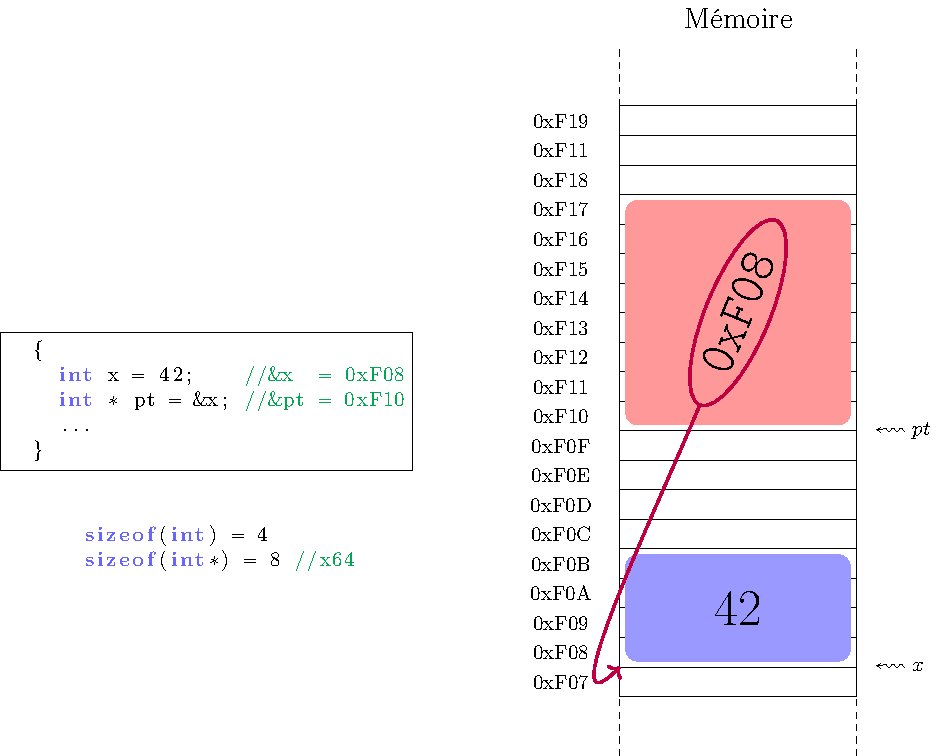
\includegraphics[width=8cm]{pics/ptr.pdf}
\end{center}
\end{frame}

\begin{frame}
\frametitle{Pointeur nuls}
\begin{itemize}[<+->]
\item On peut créer des pointeurs nuls
	\begin{itemize}
	\item En \texttt{C} : \lstinline|NULL|
	\item En \cpp\ : \lstinline|nullptr|
	\end{itemize}
\item \lstinline|NULL| est une macro : \lstinline|\#define NULL 0|
\item \lstinline|nullptr| est un immédiat
\item Déférencer un pointeur nul a un comportement indéterminé
\item Créer un pointeur n'alloue pas de mémoire vers la zone pointée
	\begin{enumerate}
	\item \lstinline|int * p;| n'alloue pas \lstinline|sizeof(int)| bytes en mémoire pour \texttt{*p}
	\end{enumerate}
\item Pour qu'un pointeur référence de la mémoire allouée, il faut soit
	\begin{itemize}
	\item que l'emplacement référencé soit pré-alloué
	\item allouer un espace dynamiquement
	\end{itemize}
\end{itemize}
\end{frame}

\begin{frame}
\frametitle{Conversions}
\begin{itemize}[<+->]
\item Conversions implicites de \texttt{T*} vers \lstinline|void*|
\item Aucune autre conversion implicite entre pointeurs n'est possible
\item Pas de conversion de \lstinline|int| vers \texttt{T*}, «~sauf~» avec \lstinline|NULL|
\end{itemize}
\begin{block}<+->{Hygiène de programmation}
	\begin{itemize}[<+->]
	\item N'utilisez jamais \lstinline|NULL| en \cpp
		\begin{itemize}
		\item \lstinline|nullptr| ne permet pas de conversions implicites
		\end{itemize}
	\end{itemize}
\end{block}
\end{frame}

\begin{frame}[containsverbatim]
\frametitle{Exemple}
\begin{itemize}
\item Fichier \texttt{ptr.c}
\end{itemize}
\begin{lstlisting}
int main() {
    int i = 3; int * pti = &i;

    printf("i = %d, pti ( %p ) : %d\n", i, pti, *pti);
    printf("Pointer address : %p of size %lu\n", &pti, sizeof(pti));

    i++;
    printf("i = %d, pti ( %p ) : %d\n", i, pti, *pti);

    double d = 2.5; double * ptd = &d;
	
    //pti = ptd; //Error
    pti = (int*)ptd; //Ok, but bad idea
    f(NULL); //Ok
    *pti = *ptd;

    int * ptn = NULL; //int * ptn = 0; //same stuff
    int * ptinv1;
    int * ptinv2 = 3; //Ok, but bad idea

    printf("%d\n", *ptn);
    printf("%d\n", *ptinv1); //bad idea
}
\end{lstlisting}
\begin{itemize}
\item Quelques différences en \cpp\ (\texttt{ptr.cpp})
\end{itemize}
\end{frame}

\begin{frame}
\frametitle{Syntaxe pointeurs et constantes}
\begin{exampleblock}<+->{Pointeur constant de \texttt{double}}
	\begin{itemize}[<+->]
	\item \lstinline|double d = 2;|
	\item \lstinline|double * const pt = &d;|
	\end{itemize}
\end{exampleblock}
\begin{exampleblock}<+->{Pointeur de \texttt{double} constant}
	\begin{itemize}[<+->]
	\item \lstinline|const double d = 2;|
	\item \lstinline|const double * pt = &d;|
	\end{itemize}
\end{exampleblock}
\begin{exampleblock}<+->{Pointeur constant de \texttt{double} constant}
	\begin{itemize}[<+->]
	\item \lstinline|const double d = 2;|
	\item \lstinline|const double * const pt = &d;|
	\end{itemize}
\end{exampleblock}
\end{frame}

\begin{frame}[containsverbatim]
\frametitle{Illustration}
\begin{itemize}
\item Fichier \texttt{ptr-cst.c}
\end{itemize}
\begin{lstlisting}
int main()
{
	int i = 2;
	const int ci = 3; //int const ci = 3 similaire
	i += 2;
	//ci += 2; //ko

	int * pi = &i; 
	printf("%p : %d\n", pi, i);
	*pi = 3; 
	printf("%p : %d\n", pi, i);

	int * const cpi = &i; //ptr constant
	*cpi = 5;
	//cpi++;

	const int * pic = &ci; //ptr d'entier constant	
	//*pic = 4;	
	pic++;

	const int * const cpic = &ci; //ptr cst d'entier cst
	//*cpic = 4;	
	//cpic++;
}
\end{lstlisting}
\end{frame}

\begin{frame}
\frametitle{Arithmétique}
\begin{itemize}[<+->]
\item On peut « déplacer » un pointeur
	\begin{itemize}
	\item C'est une adresse : on se déplace en mémoire
	\end{itemize}
\item Si \texttt{pt} est un pointeur de type \texttt{T}, alors \texttt{t + k} déplace l'adresse de \lstinline|k * sizeof(T)| bytes
	\begin{itemize}
	\item \texttt{pt++} déplace \texttt{pt} de \lstinline|sizeof(T)|
	\end{itemize}
\end{itemize}
\end{frame}

\begin{frame}[containsverbatim]
\frametitle{Illustration}
\begin{itemize}
\item Fichier \texttt{adv-ptr.c}
\end{itemize}
\begin{lstlisting}
#include <stdio.h>

void increment_and_print(int* ptr, unsigned count)
{
    for(unsigned i = 0; i < count; i++)
    {
        long long unsigned before = (long long)ptr;
        ptr++;
        printf("adress : %p shifted by %llu bytes", ptr, (long long)ptr - before);
        printf("because sizeof(int) is %zu bytes\n", sizeof(int));
    }
}

int main()
{
    int i = 0;
    int* ptr = &i;
    printf("adress before : %p\n", ptr);
    
    increment_and_print(ptr, 3); //DO NOT deference anymore    
}
\end{lstlisting}
\end{frame}

\begin{frame}[containsverbatim]
\frametitle{Application}
\begin{itemize}
\item Fichier \texttt{print-str.c}
\end{itemize}
\begin{lstlisting}
void print_str(const char* s)
{
	const char* pt = s;
	while(*pt != '\0')
	{
		printf("%c", *pt); 
		pt++;
	}
}

int main()
{
	const char* s = "Hello World!\n";
	print_str(s);
}
\end{lstlisting}
\end{frame}

\begin{frame}[containsverbatim]
\frametitle{Pointeurs vers des temporaires}
\begin{alertblock}{Attention}
	\begin{itemize}
	\item Ne retournez pas de pointeurs vers une variable locale
	\end{itemize}
\end{alertblock}
\begin{lstlisting}
int * f()
{
	int i = 2;
	return &i;
}

int main()
{
	printf("%d\n", *f()); //undefined behaviour
}
\end{lstlisting}
\end{frame}

\begin{frame}
\frametitle{Conclusion}
\begin{itemize}[<+->]
\item Les pointeurs sont des adresses
\item On peut construire un pointeur par affectation ou par prise d'adresse (\texttt{\&} préfixé)
\item On accède au contenu pointé par déférencement (\texttt{*} préfixé)
\item On dispose d'une arithmétique de pointeur pour avancer en mémoire
\item Un pointeur peut être nul
\end{itemize}
\begin{block}<+->{Hygiène de programmation}
	\begin{itemize}[<+->]
	\item N'utilisez \emph{jamais} \lstinline|NULL| en \cpp
	\end{itemize}
\end{block}
\end{frame}

\section{Pointeurs et tableaux}

\begin{frame}
\frametitle{Absence de conteneur}
\begin{itemize}[<+->]
\item En \texttt{C}, il n'existe pas de conteneurs standards	
\item Utilisation de tableaux «~en dur~», avec des pointeurs
\item La taille du tableau doit pouvoir être déterminée à la compilation
	\begin{itemize}
	\item Mention explicite
	\end{itemize}
\item Le type \texttt{type[]} est implicitement converti vers \texttt{type*} quand
	\begin{itemize}
	\item ce n'est pas un opérande de \texttt{sizeof} et \texttt{\&} (prise d'adresse)
	\item ce n'est pas un littéral de chaîne de caractère
	\end{itemize}
\item En \texttt{C}, les tableaux «~n'embarquant pas leur taille~»
	\begin{itemize}
	\item Il faut la spécifier quand on en a besoin
	\item En \cpp, on utilise des conteneurs
	\end{itemize}
\item Les éléments « non spécifiés » sont initialisés à zéro
	\begin{itemize}
	\item Si on spécifie plus d'éléments que la taille explicite : erreur
	\end{itemize}
\end{itemize}
\end{frame}

\begin{frame}[containsverbatim]
\frametitle{Syntaxe : exemple}
\begin{itemize}
\item Fichier \texttt{tab.c}
\end{itemize}
\begin{lstlisting}
long unsigned sneaky(int array[])
{
	return sizeof(array) / sizeof(*array);
}

int main()
{
	int t1[5] = {1,2,3,4};
	int t2[] = {1,2,3,4,5};
	int * t3 = t2;
	//int t4[]; 
	//int t5[5] = {1,2,3,4,5,6}; 
	int t6[8];
	
	for(int i = 0; i < 5; i++)
		printf("%d %d %d %d\n", t1[i], t2[i], t3[i], t6[i]);
		
	printf("%lu\n", sizeof(t6) / sizeof(*t6));
	printf("%lu\n", sneaky(t6));
}
\end{lstlisting}
\end{frame}

\begin{frame}
\frametitle{Tableau en mémoire}
\begin{itemize}[<+->]
\item Les données d'un tableau sont allouées de manière contiguë en mémoire
\item Même dans un tableau à plusieurs dimensions
\item On peut y accéder à partir de l'adresse du premier élément
	\begin{itemize}
	\item \lstinline|int * t = \{2,3,1,0,9,4,7,8\};|
	\item L'adresse du $4$ (6e élément) est égal à \lstinline|(t + 5)|
	\end{itemize}
\end{itemize}
\end{frame}

\begin{frame}
\frametitle{Illustration}
\begin{center}
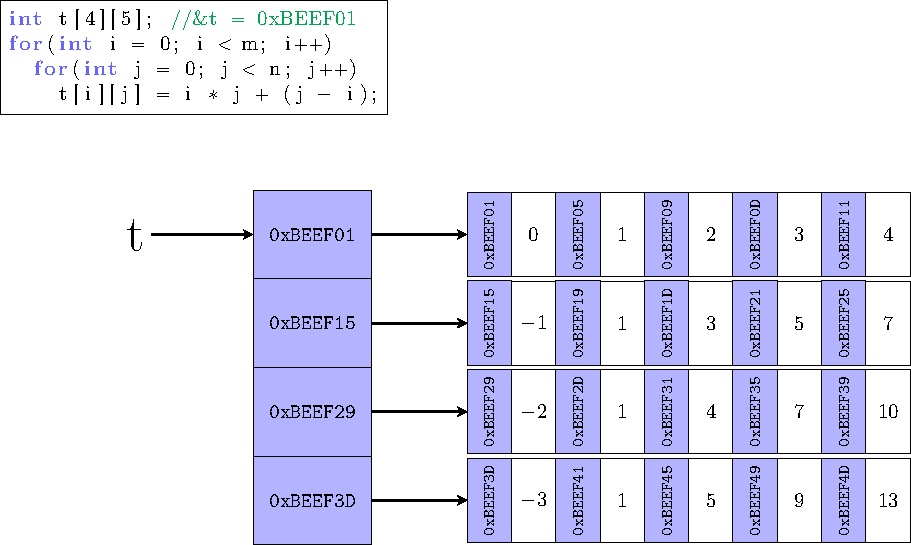
\includegraphics[width=.9\textwidth]{pics/tab.pdf}
\end{center}
\end{frame}

\begin{frame}
\frametitle{Conclusion}
\begin{itemize}[<+->]
\item On peut modéliser des tableaux à l'aide de pointeurs
\end{itemize}
\begin{block}<+->{Hygiène de programmation}
	\begin{itemize}[<+->]
	\item On utilise cela uniquement en \texttt{C} pur
	\end{itemize}
\end{block}
\begin{itemize}[<+->]
\item On accéder aux éléments à l'aide de l'opérateur \texttt{[]}, ou à partir de l'adresse du premier élément
\item La taille des tableaux doit être connue à la compilation
\end{itemize}
\end{frame}

\section{Pointeurs de fonctions}

\begin{frame}
\frametitle{Adresse d'une fonction}
\begin{itemize}[<+->]
\item Les fonctions ont des adresses dans le segment \texttt{.text}
\item On peut donc créer des pointeurs de fonction
\item Utile pour passer une fonction en paramètre d'une autre fonction
\end{itemize}
\begin{exampleblock}<+->{Syntaxe}
	\begin{itemize}[<+->]
	\item \texttt{ReturnType (*Name)(parameters)}
	\item \lstinline|void (*my_ptr)(int)| : \texttt{my\_ptr} est un pointeur de fonction prenant en paramètre un \lstinline|int| et retournant un \lstinline|void|
	\end{itemize}
\end{exampleblock}
\begin{itemize}[<+->]
\item En \cpp, il existe divers wrappers
\end{itemize}
\end{frame}

\begin{frame}[containsverbatim]
\frametitle{Exemple}
\begin{itemize}
\item Fichier \texttt{fct-ptr.c}
\end{itemize}
\begin{lstlisting}
void f(int a) 
{ 
	printf("a = %d\n", a); 
} 

int main() 
{ 
	void (*ptr)(int) = &f;
	//void (*ptr)(int) = f; //similar	

	//Function call
	(*ptr)(10); 
	//ptr(10);
} 
\end{lstlisting}
\end{frame}

\begin{frame}[containsverbatim]
\frametitle{Exemple d'utilisation}
\begin{itemize}
\item Fichier \texttt{foreach.c}
\end{itemize}
\begin{lstlisting}
void foreach_ro(int tab[], int size, void (*f)(int)) {
	for(int i = 0; i < size; i++)
		f(tab[i]);
}

void foreach_rw(int tab[], int size, int (*f)(int)) {
	for(int i = 0; i < size; i++)
		tab[i] = f(tab[i]);
}

void print(int i) {
	printf("%d ", i);
}

int increment(int i) {
	return i + 1;
}

int main() {
	int tab[] = {1,2,3,4,5};
	
	foreach_rw(tab, 5, increment);
	foreach_ro(tab, 5, print);
	printf("\n");
}
\end{lstlisting}
\end{frame}

\begin{frame}
\frametitle{Remarques}
\begin{itemize}[<+->]
\item On ne peut pas allouer ou désallouer de la mémoire à l'aide d'un pointeur de fonction
	\begin{itemize}
	\item Le segment \texttt{.text} est en lecture seule
	\end{itemize}
\item On peut créer des tableaux de pointeurs de fonction
	\begin{itemize}
	\item \lstinline|void (*my_fct_array[])(int)|
	\end{itemize}
\item Les pointeurs de fonctions permettent d'éviter la redondance de code
	\begin{itemize}
	\item \texttt{qsort}
	\item Comparateurs
	\end{itemize}
\item Si on imprime les bytes correspondant au pointeur de fonction, on obtient le langage machine
	\begin{itemize}
	\item Très utilisé en cybersécurité
	\end{itemize}
\end{itemize}
\end{frame}

\begin{frame}[containsverbatim]
\frametitle{Exemple}
\begin{itemize}
\item Fichier \texttt{machine.c}
\end{itemize}
\begin{lstlisting}
#include <string.h>

//code assembleur pour l'appel système execve sur /bin/sh
const char assembly[] = 
	"\x31\xc0\x50\x68//sh\x68/bin"
	"\x89\xe3\x50\x53\x89\xe1\x99"
	"\xb0\x0b\xcd\x80";

int main()
{
	char buffer[sizeof(assembly)];
	strcpy(buffer, assembly);

	void (*f)() = (void (*)())buffer; //living the dream
	f();
}
\end{lstlisting}
\begin{itemize}
\item Il faut compiler comme \texttt{gcc -z execstack -o machine machine.c} sur une machine non protégée
\end{itemize}
\end{frame}

\end{document}
